\chapter{Artifact design and features}
\label{Chapter5} 

In this chapter, the critical thought processes and decisions 
that shape the application architecture are documented. 
By exploring this chapter, readers will gain insights into the rationale behind the artifact structure and the reasons for selecting particular solutions over others.

\section{Capabilities and Requirements} 
\label{Requirements}

Requirements for the practical part of the thesis are defined before designing the artifact, following the DSR protocols. 
These are typically categorized into functional and non-functional requirements. 
Each plays a crucial role in the development process, 
contributing to the overall usability and performance of the application.

\subsection{Capabilities}

Use cases and requirements are added to the design of the 
artifact in the beginning to give an idea about the application's capabilities at first. 
This determines the starting point for model design. 
This definition is loosely written on paper at first and then reworked into 
requirements in cooperation with the organization introduced in section \ref{background-section}. 
The loose capabilities the application should have are as follows.
The artifact should be able to store templates for report creation. 
That means it should allow users to create templates or models to base their reports on. 
These templates should include information on how to get data and compute KPIs. 
To meet the requirement of creating custom KPIs, there has to be functionality available to create and manage custom KPIs.
The application should also provide the possibility to create graphical dashboards to 
present reports. 
Reports should also be comparable to other reports. 
Users should be able to manage who has access to their templates 
and what actions they can take in the context of their templates. 
The user creation and authentication are not handled by the application itself. 
Users are allowed to authenticate using OAUTH\footnote{https://oauth.net/2/}.

\subsection{Functional Requirements}

Functional requirements are specific and describe the expected behavior of the artifact. 
They focus on what the system should do and include specifications of operations 
to take and outcomes to expect. 
This includes user interaction or interaction with other systems if needed. 
These types of requirements are typically captured from use cases. 
Initially, the requirements were not as detailed. 
After the artifact was completed, additional specifics were included in the requirements. 
This was done to ensure that the quality assurance process could be conducted with precision,
especially when examining the user interface. 
Users can be categorized into three different roles.
The three roles are Reader, Writer, and Admin. 
A higher-ranking role inherits the privileges of the roles below it. 
For instance, an Admin has all the rights of a Writer,
and a Writer possesses all the capabilities of a Reader.
For the artifact created in this thesis, these will include: 

\compactSection{Log in}
\compactDescription{A Reader should be redirected to a login form on application startup. This form will allow the user to log in and guide them through the process. Once logged in, the user is redirected to the landing page.}
\compactSteps{
    \item Open the URL to the web application.
    \item Fill out the login form.
}
\compactOutcome{The Reader should be authenticated and redirected to the landing page.}

\compactSection{Get my models}
\compactDescription{A Reader should be able to retrieve all of their models and data. On a specific page of the application, all of the user's models are displayed in a table. There should be no model missing that the user has access to. There shouldn't be any models the user doesn't have access to.}
\compactSteps{
    \item Open the URL to the web application.
    \item Login.
    \item Go to the 'analysis' page.
    \item View the list of models.
}
\compactOutcome{The Reader should see all of their analysis models.}

\compactSection{Create a new model}
\compactDescription{The Reader should have the ability to create a new analysis model. If a new model is created, the user is automatically associated with the model as an administrative user.}
\compactSteps{
    \item Open the URL to the web application.
    \item Login.
    \item Go to the 'analysis' page.
    \item Click on 'Add a new model'.
    \item Select the new model.
    \item Click on 'Details'.
    \item Click on the tab 'Access'.
}
\compactOutcome{The Reader should now have a new model. The table under 'Access' only shows the user itself and that the Reader now has administrative privileges.}

\compactSection{View details of a model}
\compactDescription{Given a model, the Reader should be able to navigate to a detailed view of the model. This can be done by clicking a button.}
\compactSteps{
    \item Open the URL to the web application.
    \item Login.
    \item Go to the 'analysis' page.
    \item Select a model.
    \item Click on 'Details'.
}
\compactOutcome{The Reader should see a detailed page of their model.}

\compactSection{Change the KPI structure of a model}
\compactDescription{Given a model, an Editor should be able to create new KPIs, add new folders, and rename folders.}
\compactSteps{
    \item Open the URL to the web application.
    \item Login.
    \item Go to the 'analysis' page.
    \item Select a model.
    \item Click on 'Details'.
    \item Click on tab 'KPIs'.
    \item Click on 'Add new KPI'.
    \item Click on 'Add new folder'.
    \item Edit the name of a folder by clicking on the edit icon to the right of its name.
}
\compactOutcome{The Editor should be able to execute these steps without any errors.}

\compactSection{Delete a KPI or folder}
\compactDescription{Given a model, the Admin should be able to delete KPIs and folders. If a folder that contains KPIs is deleted, it should also delete the KPIs inside it.}
\compactSteps{
    \item Open the URL to the web application.
    \item Login.
    \item Go to the 'analysis' page.
    \item Select a model.
    \item Click on 'Details'.
    \item Click on tab 'KPIs'.
    \item Select a KPI.
    \item Delete the KPI.
    \item Delete a folder containing KPIs.
    \item KPI and the folder should be gone.
}
\compactOutcome{The Admin should be able to execute these steps without any errors.}

\compactSection{Edit KPI details}
\compactDescription{Given a model, the Editor should be able to edit the details of a given KPI.}
\compactSteps{
    \item Open the URL to the web application.
    \item Login.
    \item Go to the 'analysis' page.
    \item Select a model.
    \item Click on 'Details'.
    \item Click on tab 'KPIs'.
    \item Select an existing KPI or create a new KPI.
    \item Click on 'Details'.
    \item Edit the KPI name by clicking on the edit icon next to its name.
    \item Open the KPIs settings by switching to the 'Configuration' tab.
    \item Change the KPIs settings ('Basics' and 'Acceptable Items').
    \item Reload the web page.
}
\compactOutcome{The values after a page reload should be the values the Editor entered.}

\compactSection{Edit KPI expression}
\compactDescription{Given a model, the Editor should be able to edit the expression of a given KPI.}
\compactSteps{
    \item Open the URL to the web application.
    \item Login.
    \item Go to the 'analysis' page.
    \item Select a model.
    \item Click on 'Details'.
    \item Click on tab 'KPIs'.
    \item Select an existing KPI or create a new KPI.
    \item Click on 'Details'.
    \item Edit the KPIs expression by changing the type and changing the properties of the expression.
    \item Click on 'Save'.
    \item Reload the web page.
}
\compactOutcome{The values after a page reload should be the values the Editor entered.}

\compactSection{Add and edit a graphical dashboard}
\compactDescription{Given a model, the Editor should be able to add custom graphical dashboards to display report data.}
\compactSteps{
    \item Open the URL to the web application.
    \item Login.
    \item Go to the 'analysis' page.
    \item Select a model.
    \item Click on 'Details'.
    \item Click on the tab 'Settings'.
    \item Click on 'Add a new graphical layout'.
    \item A new layout should be visible in the list.
    \item Select the new layout.
    \item Click on 'Details'.
    \item Click on 'Change layout'.
    \item Add new widgets, resize, and reposition them.
}
\compactOutcome{The Editor should be able to execute these steps without any errors.}

\compactSection{Delete a graphical dashboard}
\compactDescription{Given a model, the Admin should be able to delete custom graphical dashboards.}
\compactSteps{
    \item Open the URL to the web application.
    \item Login.
    \item Go to the 'analysis' page.
    \item Select a model.
    \item Click on 'Details'.
    \item Click on the tab 'Settings'.
    \item Select a layout.
    \item Click on 'Delete'.
}
\compactOutcome{The deleted item should not show up in the list, even after a page reload.}

\compactSection{Create a report}
\compactDescription{Given a model, the Editor should be able to create a report.}
\compactSteps{
    \item Open the URL to the web application.
    \item Login.
    \item Go to the 'analysis' page.
    \item Select a model.
    \item Click on 'Details'.
    \item Switch to tab 'Reports'.
    \item Click on 'Create report'.
    \item Follow the steps to create a report.
}
\compactOutcome{The application should guide the Editor to create a report and the report should show up in the list once completed.}

\compactSection{View a report}
\compactDescription{Given a model, the Editor should be able to view a report in different ways.}
\compactSteps{
    \item Open the URL to the web application.
    \item Login.
    \item Go to the 'analysis' page.
    \item Select a model.
    \item Click on 'Details'.
    \item Switch to tab 'Reports'.
    \item Select a report.
    \item Click on 'Details'.
}
\compactOutcome{Multiple tabs feature different views of the report including a tabular view of all KPIs and a graphical view containing all configured dashboards.}

\compactSection{Delete a report}
\compactDescription{Given a model, the Admin should be able to delete a report.}
\compactSteps{
    \item Open the URL to the web application.
    \item Login.
    \item Go to the 'analysis' page.
    \item Select a model.
    \item Click on 'Details'.
    \item Switch to tab 'Reports'.
    \item Select a report.
    \item Click on 'Delete'.
}
\compactOutcome{The report is no longer listed on the model.}

\compactSection{Add a user to a model}
\compactDescription{Given a model, the Admin should be able to associate additional users to the model.}
\compactSteps{
    \item Open the URL to the web application.
    \item Login.
    \item Go to the 'analysis' page.
    \item Select a model.
    \item Click on 'Details'.
    \item Switch to the tab 'Access'.
    \item Click on 'Add user to model'.
    \item Enter the email address of the user you want to add.
}
\compactOutcome{Either the user is added to the list of associated users or a message is displayed that the user gets access to the model on the next login (If the user does not yet exist in the database he automatically gets access when they create their account).}

\compactSection{Change a user's permissions on a model}
\compactDescription{Given a model, the Admin should be able to change a user's permissions on the model.}
\compactSteps{
    \item Open the URL to the web application.
    \item Login.
    \item Go to the 'analysis' page.
    \item Select a model.
    \item Click on 'Details'.
    \item Switch to the tab 'Access'.
    \item Select a user.
    \item Click on the permission value.
    \item Select a new permission for the user.
}
\compactOutcome{The user's permissions have changed and they are only able to perform actions that are included in their permission.}

\compactSection{Remove a user from a model}
\compactDescription{Given a model, the Admin should be able to remove another user's access to the model.}
\compactSteps{
    \item Open the URL to the web application.
    \item Login.
    \item Go to the 'analysis' page.
    \item Select a model.
    \item Click on 'Details'.
    \item Switch to the tab 'Access'.
    \item Select a user.
    \item Click on 'Remove from model'.
}
\compactOutcome{The user is removed from the model and does not have access anymore.}

\subsection{Non functional Requirements}

Nonfunctional requirements are concerned with how the system performs under specific conditions. 
They do not directly capture specific functionalities but are essential in 
judging the usability, reliability, and performance of the system. 
For evaluating this later in chapter \ref{Chapter6}, a survey is crafted and distributed among the first users. 
The survey contains the questions listed in table \ref{tab:non-func-req}.

\begin{table}[!h]
    \centering
    \begin{tabular}{p{8cm} p{6cm}}
    \hline
        \textbf{Question} & \textbf{Answer options} \\ 
     \hline
        \textbf{Performance} & \\
        How would you rate the speed of the application? & 1 (Very slow) - 5 (Very fast) \\
        Did you experience any lag or delays while using the application? & 1 (Always) - 5 (Never) \\
     \hline
        \textbf{Usability} & \\
        How easy was it to navigate through the application? & 1 (Very difficult) - 5 (Very Easy) \\
        Were the instructions and labels within the application clear and understandable? & 1 (Not clear at all) - 5 (Very clear) \\
     \hline
        \textbf{Reliability} & \\
        How often did the application freeze? & 1 (Always) - 5 (Never) \\
        Were there any features or functions that did not work as expected? & Yes (please specify), No \\
     \hline
        \textbf{Security} & \\
        Did you encounter any security or privacy issues? & Yes (please specify), No \\
     \hline
        \textbf{Compatibility} & \\
        What browser did you use to access the application? & Chrome, Edge, Opera, Firefox, Other (please specify) \\
        How well did the application work on your device and operating system? & 1 (Very poorly) - 5 (Very well) \\
     \hline
        \textbf{Overall experience} & \\
        Overall, how satisfied are you with the application? & 1 (Very dissatisfied) - 5 (Very satisfied) \\
        What improvements, if any, would you suggest to enhance the application’s performance, security, or usability? & Text \\
        
    \end{tabular}
    \caption{Survey questions for nonfunctional requirements}
    \label{tab:non-func-req}
\end{table}

\section{Use cases}

Use cases of the application are defined in advance to help evaluate 
the produced artifact in the end. 
These use cases can be viewed as functional requirements that 
will be tested during the evaluation. 
The figures \ref{fig:use-cases-reader}, \ref{fig:use-cases-write} 
and \ref{fig:use-cases-admin} visualize each scenario for the three unique roles: Admin, Writer and Reader. 


All use cases are associated with requirements. 
They either have the same name as the requirement they represent or are annotated with the requirement that includes them in brackets behind their name.

\begin{figure}[!h]
    \centering
    \begin{tikzpicture}
      
        % Actor
        \umlactor[x=0, y=4]{Reader}
        
        % Use Cases Reader
        \umlusecase[x=6, y=7, name=getMyModels]{Get my Models}
        \umlusecase[x=6, y=6, name=getModelById]{View details of a model}
        \umlusecase[x=6, y=5, name=createModel]{Create a new Model}
        \umlusecase[x=6, y=4, name=getCustomQueries]{Get Custom Queries}
        \umlusecase[x=6, y=3, name=getRequiredQueries]{Get Required Queries}
        \umlusecase[x=6, y=2, name=getReport]{View a report}
        \umlusecase[x=6, y=1, name=logIn]{Log in}   
    
        
        % Associations
        \umlassoc{Reader}{getMyModels}
        \umlassoc{Reader}{getModelById}
        \umlassoc{Reader}{createModel}
        \umlassoc{Reader}{getCustomQueries}
        \umlassoc{Reader}{getRequiredQueries}
        \umlassoc{Reader}{logIn}
        \umlassoc{Reader}{getReport}
    \end{tikzpicture}
    \caption{Reader use cases of the application}
    \label{fig:use-cases-reader}
\end{figure}


\begin{figure}
    \centering
    \begin{tikzpicture}
      
        % Actor
        \umlactor[x=0, y=-3]{Writer}

        % Use Cases Writer
        \umlusecase[x=6, y=0, name=updateModel]{Update Model}
        \umlusecase[x=6, y=-1, name=createReport]{Create a report}
        \umlusecase[x=6, y=-2, name=createKPI]{Create KPI (Change the KPI structure of a model)}
        \umlusecase[x=6, y=-3, name=createLayout]{Create graphical layout (Add and edit a graphical dashboard)}
        \umlusecase[x=6, y=-4, name=updateKPI]{Update KPI (Edit KPI details)}
        \umlusecase[x=6, y=-5, name=addExpression]{Add Expression (Edit KPI Expression)}
        \umlusecase[x=6, y=-6, name=updateExpression]{Update Expression (Edit KPI Expression)}    
        \umlusecase[x=6, y=-7, name=updateLayout]{Update graphical layout (Add and edit a graphical dashboard)}
        
        % Associations
        \umlassoc{Writer}{updateModel}
        \umlassoc{Writer}{createReport}
        \umlassoc{Writer}{createKPI}
        \umlassoc{Writer}{createLayout}
        \umlassoc{Writer}{updateKPI}
        \umlassoc{Writer}{addExpression}
        \umlassoc{Writer}{updateExpression}
        \umlassoc{Writer}{updateLayout}
    \end{tikzpicture}
    \caption{Writer use cases of the application}
    \label{fig:use-cases-write}
\end{figure}

\begin{figure}
    \centering
    \begin{tikzpicture}
      
        % Actor
        \umlactor[x=0, y=-8]{Admin}

        % Use Cases Admin
        \umlusecase[x=6, y=-6, name=deleteKPI]{Delete KPI or folder}
        \umlusecase[x=6, y=-7, name=deleteReport]{Delete a report}
        \umlusecase[x=6, y=-8, name=deleteLayout]{Delete a graphical dashboard}
        \umlusecase[x=6, y=-9, name=addUser]{Add a user to a model}
        \umlusecase[x=6, y=-10, name=deleteUser]{Remove a user from a model}
        \umlusecase[x=6, y=-11, name=updateUser]{Change a user's permissions on a model}     
    
        
        % Associations
        \umlassoc{Admin}{deleteReport}
        \umlassoc{Admin}{deleteKPI}
        \umlassoc{Admin}{deleteLayout}
        \umlassoc{Admin}{addUser}
        \umlassoc{Admin}{deleteUser}
        \umlassoc{Admin}{updateUser}
    \end{tikzpicture}
    \caption{Admin use cases of the application}
    \label{fig:use-cases-admin}
\end{figure}


\newpage

\section{Model}

This section dives into the system's structure and its intended operations. 
First, the model is presented, detailing the primary components. 
Following that, various use cases illustrate the system in action, providing a comprehensive understanding of its functionality and interactions.

\subsection{Data model}

A central part of this application will be the data model behind it. 
Before actually implementing this model it is sketched out on paper. 
This step ensures that there is a clear picture of how the data elements relate and interact with each other. 
By mapping things out early, one can pinpoint potential issues and make necessary adjustments. 
Essentially, it's about laying a strong foundation from the get-go to ensure the app's long-term efficiency and adaptability. 
When the sketch is finished the model will be implemented code-first using an ORM tool to map the coded model into a relational database. 

Most models will have a property called \code{Id} in which they store a GUID value as the primary key for the relational database mapping. 
The diagrams presented in this section were designed with the UML standard \footnote{\cite{uml_standard}} in mind. 
However, it is worth noting that while every effort is made to comply with the UML conventions there might be subtle differences in the representation. 

\begin{figure}
    \centering
    
        \begin{tikzpicture}
          
         \styledumlclass{AnalysisModel}{
          + Id : Guid \\
          + Name : string \\
          + ModelUsers : List<UserModel> \\
          + KPIs : List<KPI> \\
          + KPIFolders : List<KPIFolder> \\
          + Reports : List<Report> \\
          + Graphical : List<GraphicalConfiguration> \\
        }{}{0}{0}
        
        \styledumlclass{Expression}{
          + Id : Guid \\
          + Type : ExpressionType \\
          + ALLOWED\_QUERY\_TYPES : List<QueryReturnType> \\
          + QueryId : string \\
        }{
          + Evaluate(data : Dictionary<string, QueryResult>) : object? \\
          + GetRequiredQueries() : IEnumerable<string> \\
        }{0}{10}
        
        
        \styledumlclass{KPI}{
          + Id : Guid \\
          + Name : string \\
          + Unit : string \\
          + Expression : Expression \\
          + ShowInReport : bool \\
          + AcceptableValues : string? \\
          + AnalysisModelId : Guid? \\
          + FolderId : Guid? \\
        }{}{5}{5}
        
        \styledumlclass{KPIFolder}{
          + Id : Guid \\
          + Name : string \\
          + ParentFolderId : Guid \\
          + ModelId : Guid \\
          + KPIs : List<KPI> \\
          + SubFolders : List<KPIFolder> \\
        }{}{-5}{5}
        
        \styledumlclass{Report}{
          + Id : Guid \\
          + AnalysisModelId : Guid \\
          + Title : string \\
          + Notes : string \\
          + Created : long \\
        }{}{3}{-5}

        \styledumlclass{ReportData}{
        + Id: Guid \\
        + QueryResults: Dictionary<string, QueryResult> \\
        + KPIsAndValues: Dictionary<Guid, object?> \\
        }{}{4.25}{-10}

        \styledumlclass{GraphicalConfiguration}{
          + Id : Guid \\
          + Name : string \\
          + ModelId : Guid \\
          + Items : List<GraphicalReportItem> \\
        }{}{-4}{-5}
        
        \styledumlclass{GraphicalReportItem}{
          + Id : Guid \\
          + Type : GraphicalReportItemType \\
          + Name : string \\
          + Properties : GraphicalReportItemProperties \\
          + Layout : GraphicalReportItemLayout \\
          + DataSources : GraphicalItemDataSources \\
        }{}{-4}{-10}
        
        
        
        \umlassoc{KPI}{Expression}
        \umlaggreg{AnalysisModel}{KPI}
        \umlaggreg{AnalysisModel}{KPIFolder}
        \umlaggreg{AnalysisModel}{Report}
        \umlaggreg{AnalysisModel}{GraphicalConfiguration}
        \umlaggreg{KPIFolder}{KPI}
        \umlaggreg{KPIFolder}{KPIFolder}
        \umlaggreg{GraphicalConfiguration}{GraphicalReportItem}
        \umlassoc{Report}{ReportData}

        \end{tikzpicture}

    \caption{Relation KPIs and AnalysisModels}
    \label{fig:kpis-and-models}
\end{figure}


\subsubsection{Analysis models}

The idea of this application is to have a way to design a schema or model that can be followed to evaluate performance indicators about a SCRUM sprint. 
The \code{AnalysisModel} data class is designed to do just that. 
It holds information about how to get and evaluate data. 
It also includes configuration on how to visualize data to present it to team members. 
A graphical representation shows the most important parts of the model in figure \ref{fig:kpis-and-models} after a brief description in the next paragraphs.

KPIs are an essential part of this thesis and have to be included in the data model. 
The classes \code{KPI} and \code{Expression} are designed to store details about KPIs and how to evaluate them. 
Also included in the \code{KPI} class is the configuration of the KPI like the unit to display and if it is supposed to show up on the final report. 
If a team has a lot of KPIs to calculate, storing them in a list can become very confusing. 
That's why the class \code{KPIFolder} is introduced so that a hierarchical structure can be offered. 
This allows KPIs to be organized familiarly.

\code{Expression}s are a way of telling the software how to evaluate raw data and reduce it to a KPI value. 
For this application, a few different types of expressions suffice. 
Further information on expressions is detailed in section \ref{model-expressions}.

To save actual reports and the data collected for them the \code{Report} class is designed. 
It relates to an \code{AnalysisModel} which in turn can relate to many instances of the \code{Report} class. 
The actual report data is held by the class \code{ReportData} which has a one-to-one relationship with the \code{Report} class as illustrated in figure \ref{fig:kpis-and-models}. 
Since the shape of the data saved in a report heavily depends on the model configuration the properties \code{QueryResults} and \code{KPIsAndValues}, 
which are holding the data, are saved in the database as JSON binary data. 
This makes sure the data received when executing queries can be stored in its raw form, which in turn means that the evaluation of KPIs can be designed more flexibly. 

The class \code{GraphicalConfiguration} is used to store dashboards and layouts to display reports graphically. 
This way dashboards can be configured dynamically and presented to the team.

\begin{table}[!h]
    \centering
    \begin{tabular}{c c p{8cm}}
    \hline
    \textbf{Expression} & \textbf{Category} & \textbf{Description} \\
    \hline
    Add & Mathematical & Adds the result of two other KPIs together. \\
    \hline
    Div & Mathematical & Divides the result of two other KPIs. Useful for calculating ratios. \\
    \hline
    Multiply & Mathematical & Multiplies the result of two other KPIs. Useful to scale a value by a certain factor. \\
    \hline
    Subtract & Mathematical & Subtracts the result of two other KPIs. \\
    \hline
    Avg & Aggregation & Iterates over all list items extracting the given field. When all the values are extracted, the mathematical average is calculated. \\
    \hline
    Min & Aggregation & Iterates over all list items extracting the given field. When all the values are extracted, the mathematical minimum is calculated. \\
    \hline
    Max & Aggregation & Iterates over all work items extracting the given field. When all the values are extracted, the mathematical maximum is calculated. \\
    \hline
    Sum & Aggregation & Iterates over all work items extracting the given field. When all the values are extracted, the mathematical sum is calculated. \\
    \hline
    CountIfMultiple & Conditional & Count values in a list if they meet multiple conditions. \\
    \hline
    SumIfMultiple & Conditional & Sum values in a list if they meet multiple conditions. \\
    \hline
    CountIf & Conditional & Count values in a list if they meet a certain condition. \\
    \hline
    Plain & Atomic & Just return the plain result of a query. \\
    \hline
    Value & Atomic & Expression to define a simple numeric value. Useful for mathematical operations. \\
    \end{tabular}
    \caption{Descriptions of different expression types}
    \label{tab:expression-types}
\end{table}


\begin{figure}[!h]
    \centering
    \begin{tikzpicture}

        \styledumlclass{Expression}{
          + Id : Guid \\
          + Type : ExpressionType \\
          + QueryId: string \\
        }{
          + \textit{Evaluate(data : Dictionary<string, QueryResult>) : object?} \\
        }{0}{0}
        
        \styledumlclass{MathOperationExpression}{
            + Left: KPI \\
            + Right: KPI \\
        }{
            + \textit{DoOperation(double left, double right) : double} \\
        }{-5}{-8}
        
        \styledumlclass{AggregateExpression}{
          + Field : string \\
        }{
        }{5}{-8}
        
        \styledumlclass{DoIfMultipleExpression}{
          + Conditions : List<Condition> \\
          + Connection : ConditionConnection \\
          + ExtractField : string \\
        }{
            + \textit{Process(IEnumerable<object> conditionalItems): object?} \\
        }{0}{-12}
        
        \styledumlclass{PlainQueryExpression}{
        }{
        }{-5}{-4}

       \styledumlclass{NumericValueExpression}{
          + Value : double \\
        }{
        }{5}{-4}
        
        
        \umlinherit{MathOperationExpression}{Expression}
        \umlinherit{AggregateExpression}{Expression}
        \umlinherit{NumericValueExpression}{Expression}
        \umlinherit{DoIfMultipleExpression}{Expression}
        \umlinherit{PlainQueryExpression}{Expression}
        
        \end{tikzpicture}

    \caption{Expression types hierarchy}
    \label{fig:expression-hier}
\end{figure}


\subsubsection{Expressions}\label{model-expressions}

\code{Expression}s are tightly coupled with \code{KPI}s and are used to evaluate sprint data and reduce it to values that can be displayed in a sprint report.
There are multiple types of expressions to evaluate different KPIs described in table \ref{tab:expression-types}.
These expressions can be in one of four different categories.
A \textit{Mathematical} expression is, unsurprisingly, used for mathematical operations.
It is used to combine other KPIs to calculate numeric values.
Aggregating an array of values can be achieved by using an expression of the \textit{Aggregation} category.
These expressions can reduce an array to a single value, calculating things like the maximum, minimum or average.
A \textit{Conditional} expression is used to filter a list of values and then perform an operation on them.
This allows for KPIs to count or sum values only if they meet certain conditions.
Lastly, \textit{Atomic} expressions can be used to represent simple, hard-set values or the plain value of a query. 
These expressions are modeled as a hierarchical structure with the \code{Expression} class as a base.
Their model is illustrated in figure \ref{fig:expression-hier}.

\subsubsection{User management}

User management is crucial to an application that stores data multiple people should have access to. 
User access is controlled at the level of analysis models. 
This means a user can either have reading, writing or admin access to an \code{AnalysisModel} instance. 
Reading access privileges include read access to every related entity and the model itself.
Writing access works in the same manner and just adds writing access to all entities of the model. 
The only special access privileges are granted to administrative users. 
These allow a user to give other users access to the model and delete entities. 
Since a user can have access to multiple models and models should be able to be accessed by multiple users, an intermediate table is needed to model this relationship. 
This is illustrated in the diagram \ref{fig:user-model}.

\begin{figure}
    \centering
    \begin{tikzpicture}

        \styledumlclass{User}{
          + Id : Guid \\
          + DisplayName : string \\
          + EMail: string \\
        }{
        }{0}{3}
        
        \styledumlclass{RefreshToken}{
          + Token : string \\
          + IsActive : bool \\
        }{
        }{-5}{3}
        
        \styledumlclass{UserModel}{
          + Permission: ModelPermission \\
        }{
        }{0}{0}
        \styledumlclass{AnalysisModel}{
          + Id : Guid \\
          + Name : string \\
        }{}{-5}{0}

        \umlaggreg{AnalysisModel}{UserModel}
        \umlaggreg{User}{UserModel}
        \umlaggreg{User}{RefreshToken}
        
    \end{tikzpicture}
    
    \caption{User data model}
    \label{fig:user-model}
    
\end{figure}

\newpage

\section{Design considerations and choices}

\subsection{Implementation specifics}

There are multiple options for implementing an application to read and compile 
information from a digital SCRUM platform.
To meet the requirements of the partnering company this includes writing an extension for a 
specific platform and creating custom software that uses 
REST endpoints if the platform exposes any.

\subsubsection{Extension for a SCRUM platform}
The requirement is to produce an artifact that will be used to extract 
data from the SCRUM platform Azure DevOps. 
Therefore a viable option would be to develop an extension for this platform.
Microsoft provides documentation on how to develop extensions for your 
organizational DevOps platform \footnote{Developing extensions for Azure: https://learn.microsoft.com/en-us/azure/devops/extend/overview?view=azure-devops}.
Simple authentication for users, storage provided by Azure and the 
accessibility of use speak in favor of this method.
The only downside, why it should be decided against, is that an extension for 
DevOps limits the functionality of the application to the Microsoft platform. 
If other things would also want to be integrated in the future, 
the application could not be extended in such a way that it 
also works with external applications. 
In addition, only developers could evaluate sprints and view the 
results because a Visual Studio license is required to access the platform.

\subsubsection{Independent application}
An independent application can access work items and sprint info via a REST API provided by the most used SCRUM platforms like Atlassian Jira and Azure DevOps \parencite{TopTenScrum}.
If needed in the future, more platforms can be integrated into this 
application and it could be hosted anywhere. 
Another advantage is the free choice of the implementation language, 
which makes it much easier for a company to expand the application at a later date. 
A disadvantage is that the application has to be written from scratch. 
This means that communication with Azure services, user authentication, 
and data storage must both be designed and implemented. 
Nevertheless, it is a favorable choice.

\subsection{Application architecture}

An important decision is made to adopt a distributed application 
architecture. This is achieved by separating the front-end, back-end, and database into containerized parts. 
This choice is influenced by several factors and research pieces. 
One paper explores the performance of traditional VM deployments and 
contrasts them with the use of Linux containers. 
The authors used KVM as a representative hypervisor and Docker as a container manager. 
The results show that containers result in equal or better 
performance than VMs in almost all cases \parencite{felter2015updated}. 
Another study compares the performance of Docker containers and VMs using 
different cloud vendors. 
Docker containers are found to be faster than KVMs and Xen VMs in terms of response time, 
download time, CPU processing time, and memory usage. 
The performance of Docker containers improves when scaled using the 
Kubernetes framework \parencite{chengeta2021comparing} which will also be 
the hosting choice for first evaluating the artifact. 
Relevant to this thesis and the decision made are the following points:

\begin{itemize}
    \item \textbf{Modern technology}: Distributed applications, especially when combined with containers, represent the cutting edge in software architecture. 
    \item \textbf{Scalable components}: One of the primary advantages of a distributed application is its scalability. Although it's not important for this thesis it's nice to have the option to scale as demand gets higher.
    \item \textbf{High availability}: Distributed architectures tend to offer better fault tolerance. Containerization further enhances this by allowing rapid redeployment of single components, ensuring minimal downtime.
    \item \textbf{Resource efficiency}: Containers are lightweight compared to traditional virtual machines. This means they start quickly and use fewer system resources. Multiple containers can be deployed onto a single machine which means that resources can be used more efficiently.
    \item \textbf{Consistent environments}: Containerization ensures that the application runs the same, regardless of where the container is deployed. This consistency can reduce the "it works on my machine" type of issues. 
    \item \textbf{Personal experience}: Familiarity with the technology stack is invaluable. Having prior experience with distributed systems and containers ensured a smoother development process.
\end{itemize}

Of course, the strategy of creating an application of containerized services is not suited for every application. 
This section illustrates that this is the best choice for this specific application and the partnering companies' hosting choices.

\subsection{Programming languages and frameworks}

Selecting a programming language for a project is often influenced by the developer's previous experience. 
In many cases, developers lean towards languages they are already familiar with. 
This eliminates the need to learn a new language. 
This preference is not just a matter of comfort but also efficiency. 
Using a programming language known by the developer reduces errors, saves time,
and enhances the quality of the final artifact. 
Since the application is split into three parts two programming languages and frameworks have to be selected in addition to a database system.


\subsubsection{Back-end}

The heart of the application is its API which is used to create and evaluate KPIs, 
issue and review Reports, and define dashboards for report presentation to a SCRUM team. 
ASP.NET is selected for this part of the application, 
which is a web application framework developed by Microsoft. 
ASP.NET is built on the Common Language Runtime (CLR), 
which means developers can write ASP.NET code using any supported .NET language like C\#, 
VB.NET, and F\#. The choice for this project is to use ASP.NET with C\# \footnote{ASP.NET documentation: https://learn.microsoft.com/en-us/aspnet/core/?view=aspnetcore-7.0}.

\subsubsection{Database}

A relational database is used to store reports, 
KPIs, and other models that are needed for the application. 
The choice of provider is PostgreSQL because it's open source and easy to use with ASP.NET. 
The database schema is implemented code-first using an Object-Relational Mapping (ORM) framework for ASP.NET called Entity Framework. 
This framework automatically takes care of any migrations that may need to be issued to the schema and allows incremental creation of the model code first.

\subsubsection{Front-end}

To present sprint metrics and data, configure how data is retrieved,
and manage user access a user interface is essential.
The front end of the application is coded in Typescript with the
extended capabilities of the library React by Facebook 
\footnote{React by Facebook: \cite{ReactDev}}. 
The user interface provides a method for the user to interact with the back-end API using controls rather than web requests which makes the application more accessible.  

\subsubsection{Composition}

The final artifact consists of three docker images: 
one for the front end of the application, one for the back end,
and one for the database\footnote{Docker: \cite{DockerGetStarted}}.
Locally, this can be run via a provided 'docker-compose' file but in production,
these images need to be hosted separately and configured in such a 
way that they know each other's location.

\section{Limitations}

The artifact is designed to have very few limitations when it comes to analyzing sprint data. 
The flexibility of having custom KPIs extends the types of metrics that can be extracted 
from Sprint by a lot. Some limitations however still exist:

\subsection*{Dependencies}

The produced artifact has dependencies that limit its use. The final application may only be used with SCRUM logging software that provides some sort of API to gather data. The data that is returned by this endpoint may only have a structured form (YAML, JSON). Examples of this are Azure DevOps Boards and Atlassian Jira.

\subsection*{Multiple organisations}
Pre-deployment of the artifact requires some configuration to be able to start. Each instance of the artifact has to know which endpoint to use to gather information about sprints. This makes the use of the artifact by multiple organizations impossible since they likely have different endpoints to query. Since the artifact is published as a lightweight Docker image it should be no problem to deploy one instance per organization. 

\section{Highlighted features}

This section provides a view into some highlighted features of the artifact. 
These are features that are characterized by the fact that they are more complex than others, 
are very relevant to understanding the artifact, 
and have special functionality. 

\subsection{Retrieving sprint data dynamically}

With the requirement to be able to request data from every possible SCRUM software that has some kind of API, 
some hurdles presented themselves for the design of the application. 

APIs from different providers have different specifications and also offer different possibilities. 
For example, Azure DevOps offers the option of installing a C\# package and reading out sprint data. 
Other providers such as Atlassan Jira offer a REST API. 
So it's important to find a way to support all methods.

To give the user the most flexibility but also restrict usage in some ways, 
an interface for sprint data retrieval is designed (Listing \ref{lst:devops-interface}).

\begin{lstlisting}[style=csharp, caption=Expression base class, label=lst:devops-interface]
public interface IDevOpsProviderService
{
    // Get all available queries provided by this SCRUM software 
    List<Query> GetQueries();
    // Get details of a single query  
    Query GetQueryById(string id);
    // Get parameters for the query that the query needs before executing  
    Task<List<QueryParameter>> GetQueryRuntimeParametersAsync(string queryId);
    // Execute a single query  
    Task<QueryResult> ExecuteQueryAsync(string queryId, Dictionary<string, object?> runtimeParameterValues);
    // Checks if the service has a valid configuration  
    bool HasValidConfiguration();
}
\end{lstlisting}

This allows the programmer to create standard classes for each major SCRUM provider starting with Azure DevOps. 
Additionally, if other, non-common software should be used to retrieve data the software can be extended by implementing this interface in a custom class and switching the used class out in the dependency injection configuration (Listing \ref{lst:devops-injection}). 

\begin{lstlisting}[style=csharp, caption=Expression base class, label=lst:devops-injection]
// Create ASP.Net application
var builder = WebApplication.CreateBuilder(args);

// Add configuration
var configFile = Path.Join(builder.Environment.ContentRootPath, "appsettings.json");
builder.Configuration.AddJsonFile(configFile, optional: false);

// Configure dependency injection service

// Add database configuration
builder.Services
    .AddDbContext<DataContext>(opts =>
    {

        var connectionString =  builder.Configuration
            .GetConnectionString("PostgresDatabase")

        opts.UseNpgsql(connectionString);
    });

// Add other services
// [...]
 
// Inject Azure DevOps provider service
builder.Services.AddScoped<IDevOpsProviderService, AzureDevOpsProviderService>();

\end{lstlisting}

This allows the workflow of creating a report to be the same regardless of the provider used. The user decides to create a sprint report and clicks the button in the UI, triggering that action. The user enters the name of the report and clicks 'Next'. After that, the UI requests an API endpoint called 'GetRequiredQueries' which yields all required queries by the model to create a report. 
After this list is returned, the front end requests an endpoint 'GetQueryRuntimeParameters' for each of the queries. Each of these requests returns a List of parameters for a query. These parameters are displayed for the user in a form. The user fills out the form and clicks 'Next'. The front-end sends a request to the back-end API endpoint 'CreateReport', including the query parameter values entered by the user. The back-end creates a report and saves it to the database. The report is then returned to the UI and the user can now see it. This behavior is also illustrated in figure \ref{fig:seq-queryparameters} in the form of a sequence diagram.

\begin{figure}
    \centering
    \begin{sequencediagram}
        \newinst{user}{User}
        \newinst[3]{ui}{UI}
        \newinst[3]{backend}{Backend}
        \newinst[3]{db}{Database}

        \mess{user}{Clicks create report button}{ui}
        \postlevel
        \mess{user}{Enters report name and clicks 'Next'}{ui}
        \mess{ui}{GetRequiredQueries}{backend}
        \mess{backend}{Queries list}{ui}
        
        \postlevel
        \begin{call}{ui}{For each query}{ui}{}
        \postlevel
            \mess{ui}{GetQueryParameters}{backend}
            \mess{backend}{Parameters list}{ui}
        \end{call}
        
        \mess{ui}{Displays parameters form}{user}
        \mess{user}{Fills out form and clicks 'Next'}{ui}
        \mess{ui}{CreateReport}{backend}
        \begin{call}{backend}{Save report}{db}{}
            \mess{db}{Report saved}{backend}
        \end{call}
        
        \mess{backend}{Returns report}{ui}
        \mess{ui}{Displays report}{user}
    \end{sequencediagram}
    \caption{Sequence diagram for creating a sprint report.}
    \label{fig:seq-queryparameters}
\end{figure}

\newpage

\subsection{Model associations of non-existent users}

\begin{figure}
    \centering
    \begin{tikzpicture}

         \styledumlclass{AnalysisModel}{
          + Id : Guid \\
          + Name : string \\
          + ModelUsers : List<UserModel> \\
          + KPIs : List<KPI> \\
          + KPIFolders : List<KPIFolder> \\
          + Reports : List<Report> \\
          + Graphical : List<GraphicalConfiguration> \\
        }{}{0}{0}

        \styledumlclass{ModelAssociationRequest}{
            + Id: Guid \\
            + Email: string \\
            + IssuedBy: User \\
            + IssuedAt: long \\
            + Completed: bool \\
            + CompletedAt: bool \\
            + Permission: ModelPermission \\
        }{}{0}{-5}

        \umlaggreg{AnalysisModel}{ModelAssociationRequest}
        
        \end{tikzpicture}

    \caption{ModelReportAssociation model}
    \label{fig:model-assoc}
\end{figure}


Since users are not stored in the application database and can use OAUTH to log in, a user may not exist by the time another user wants to add them to their model. This creates a need for the capability to associate a user automatically to a model when they first log in. This is realized by a class called \code{ModelAssociationRequest} (see figure \ref{fig:model-assoc}). This class is created when a user adds a non-existing user to their model. If a new user logs in all saved \code{ModelAssociationRequests} are searched for a matching email address. If one is found, the new user is automatically associated with the model listed in the \code{ModelAssociationRequest} entity. This behavior is illustrated in listing \ref{lst:user-update-method}.

\begin{lstlisting}[style=csharp, caption=Create user method, label=lst:user-update-method]
/// Method to create and update a user (user is created if id is not found)
public async Task<User> CreateOrUpdateUserAsync(User user)
{
    var existing = await m_context.Users.FindAsync(user.Id);
    // Check if user exists
    if (existing != null)
    {
        existing.DisplayName = user.DisplayName;
        existing.EMail = user.EMail.ToLowerInvariant();
    }
    else
    {
        user.EMail = user.EMail.ToLowerInvariant();
        existing = (await m_context.Users.AddAsync(user)).Entity;
        var modelAssocRequests = await m_context.ModelAssociationRequests
            .Where(x => x.Email == user.EMail && !x.Completed).ToListAsync();
        foreach (var request in modelAssocRequests)
        {
            var model = await m_context.AnalysisModels
                .FindAsync(request.ModelId);
            // Create association from user to model
            var userModel = new UserModel 
                { 
                    Model = model, 
                    User = existing, 
                    Permission = request.Permission, 
                };
            
            await m_context.UserModels.AddAsync(userModel);

            request.Completed = true;
            request.CompletedAt = DateTime.Now.ToUnixEpochTime();
        }
    }

    await m_context.SaveChangesAsync();
    return existing;
}
\end{lstlisting}


\subsection{Dynamic dashboard layouts}

\begin{figure}
    \centering
    \begin{tikzpicture}

         \styledumlclass{AnalysisModel}{
          + Id : Guid \\
          + Name : string \\
          + ModelUsers : List<UserModel> \\
          + KPIs : List<KPI> \\
          + KPIFolders : List<KPIFolder> \\
          + Reports : List<Report> \\
          + ModelAssociationRequests : List<ModelAssociationRequest> \\
        }{}{0}{0}

        \styledumlclass{GraphicalConfiguration}{
            + Id: Guid \\
            + Name: string \\
        }{}{-4}{-5}
        
        \styledumlclass{GraphicalConfigurationItem}{
            + Id: Guid \\
            + Type: GraphicalReportItemType \\
            + Name: string \\
            + Layout: GraphicalReportItemLayout \\
            + DataSources: GraphicalItemDataSources \\
        }{}{4}{-5}
        
        \styledumlclass{GraphicalReportItemLayout}{
            + Id: Guid \\
            + X: int \\
            + Y: int \\
            + W: int \\
            + H: int \\
            + MaxW: int \\
            + MaxH: int \\
            + MinW: int \\
            + MinH: int \\
        }{}{-4}{-10}
        
        \styledumlclass{GraphicalItemDataSources}{
            + Id: Guid \\
            + KPIs : List<Guid> \\
        }{}{4}{-10}

        \umlaggreg{AnalysisModel}{GraphicalConfiguration}
        \umlaggreg{GraphicalConfiguration}{GraphicalConfigurationItem}
        \umlassoc{GraphicalConfigurationItem}{GraphicalReportItemLayout}
        \umlassoc{GraphicalConfigurationItem}{GraphicalItemDataSources}
        
        \end{tikzpicture}

    \caption{Graphical layout model}
    \label{fig:graphical-items-layout}
\end{figure}


Custom configurable KPIs also require custom display options. 
Some KPIs may be better interpreted when viewed as a graph compared to just looking at the numeric value. 
The artifact should provide the possibility to create multiple dashboards for a model and these dashboards should have configurable layouts. 
The model constructed for this purpose is described as follows: 
An \code{AnalysisModel} can include many dashboards, which are represented by the entity class \code{GraphicalConfiguration}. 
Each \code{GraphicalConfiguration} may have multiple widgets modeled by the class \code{GraphicalReportItem}. 
These items include properties that can be used to save their size and position in the dashboard. 
The dashboards expand to the lower side of the screen and have a fixed number of twelve slots in the horizontal plane. 
Each widget on the dashboard can be scaled and re-positioned. 
This means developing the model to save layouts in the database and also finding a way to implement this in the front end of the application.
The model is illustrated in figure \ref{fig:graphical-items-layout} and some visualizations of the front-end code are included in figure \ref{fig:dashboards-config}. 
An applied version of the dashboard is illustrated in figure \ref{fig:appl-dashboard}. 
The different types of widgets also determine the maximum and minimum size of the widget. 
The data sources for the widget are mostly KPIs but for easier changes in the future, these properties have been abstracted to the class \code{GraphicalItemDataSources}.

\begin{figure}
    \centering
    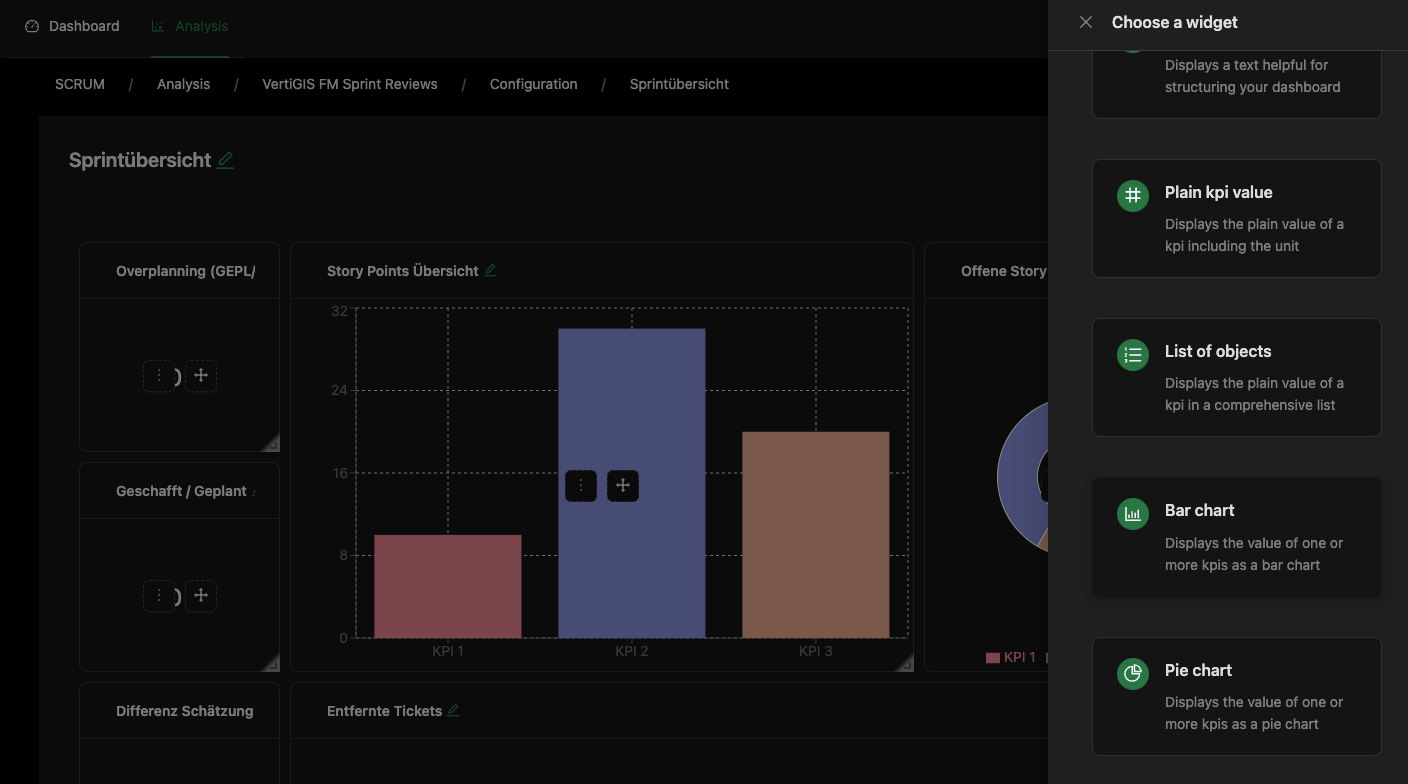
\includegraphics[width=0.6\linewidth]{Figures/DashboardsConfig.png}
    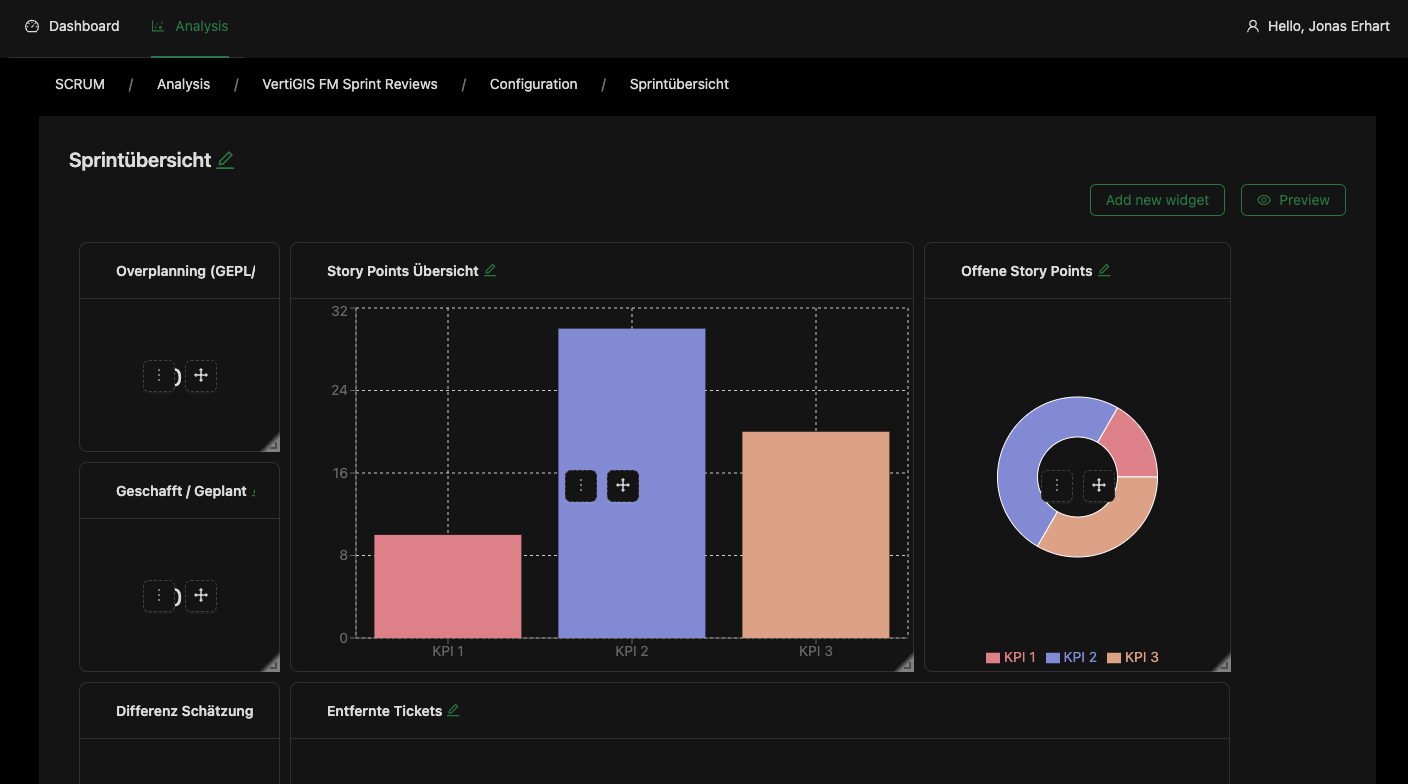
\includegraphics[width=0.6\linewidth]{Figures/DashboardConfigWidgets.png}
    \caption{Dashobard widget types and configuration}
    \label{fig:dashboards-config}
\end{figure}

\begin{figure}
    \centering
    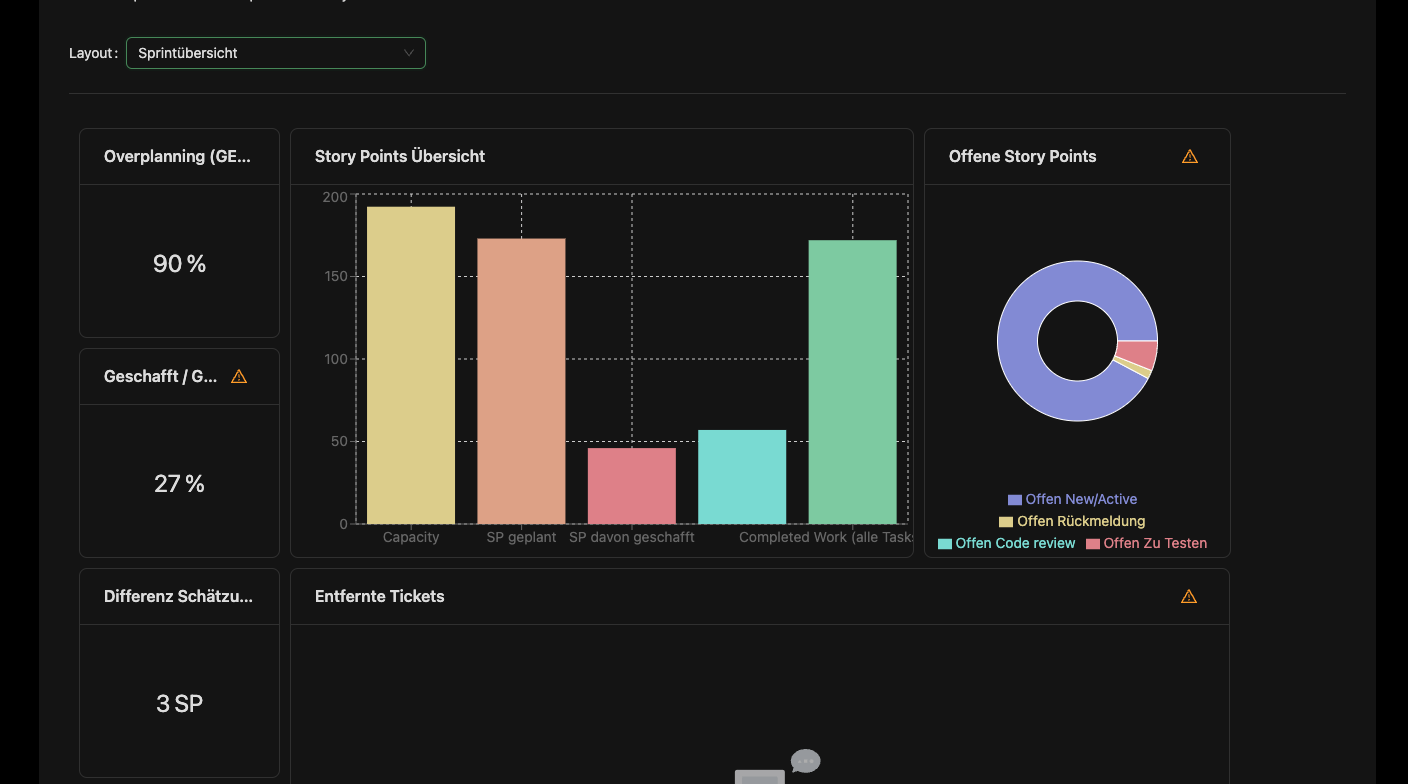
\includegraphics[width=1\linewidth]{Figures/DashboardApplication.png}
    \caption{Applied dashboard with real data}
    \label{fig:appl-dashboard}
\end{figure}
